\section{Numerical Experiments}
As the final part of our report, we implement the algorithms in the original article with \texttt{Julia} and its package \texttt{DifferentialEquations.jl} \cite{rackauckas2017differentialequations}. By comparing ODE direct discretizating (DD) methods described in the article against gradient descent (GD) and Nesterov's accelerated gradient (NAG) methods, we con verify the main results in the theoretical part.

Inspired by the numerical results by \textcite{NEURIPS2019_7a2b33c6}, we generate normal distributed separable dataset and fit a linear model \(Ax=b\). Then, we minimize three different kinds of loss functions:
\begin{equation}
    \begin{aligned}
        f_1(x) & = \left\| Ax-b \right\|_{2}^2            \\
        f_2(x) & = \log(1+e^{-y w^{\mathrm{T}}x})         \\
        f_3(x) & = \frac{1}{4}\left\| Ax-b \right\|_{4}^4
    \end{aligned}
\end{equation}
where $f_1(\cdot ),f_2(\cdot ),f_3(\cdot )$ are $L_2$ loss, logistic loss and $L_4$ loss, respectively. For each test case and optimization algorithm, we empirically select the learning rate as the largest step length among $\{ 10^{-k}|k\in \mathbb{Z} \}$ that the method remains stable during the optimization process. Main results are shown in figure \ref{Numerical} where all figures are on log-log scale.
\begin{figure}[htbp]
    \begin{subfigure}{0.4\textwidth}
        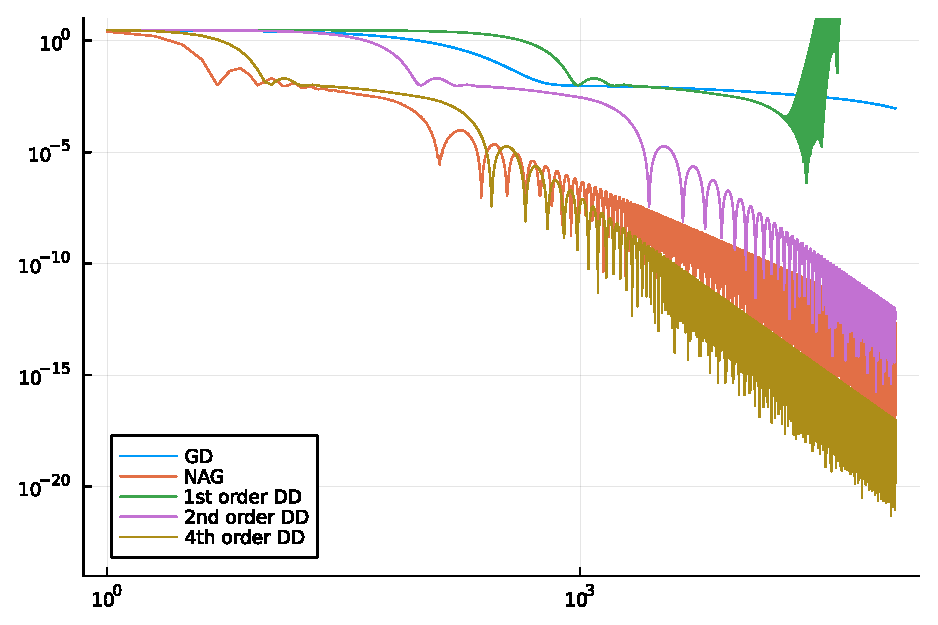
\includegraphics[width=\textwidth]{"assets/quadratic-1.pdf"}
        \caption{}
        \label{fig:l2-1}
    \end{subfigure}
    \hfill
    \begin{subfigure}{0.4\textwidth}
        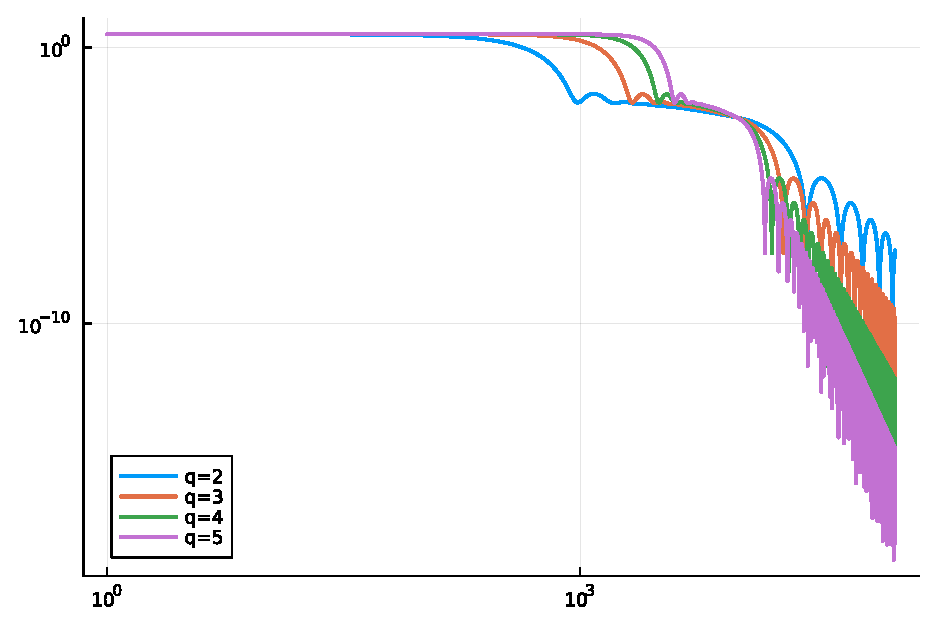
\includegraphics[width=\textwidth]{"assets/quadratic-2.pdf"}
        \caption{}
        \label{fig:l2-2}
    \end{subfigure}
    \hfill
    \begin{subfigure}{0.4\textwidth}
        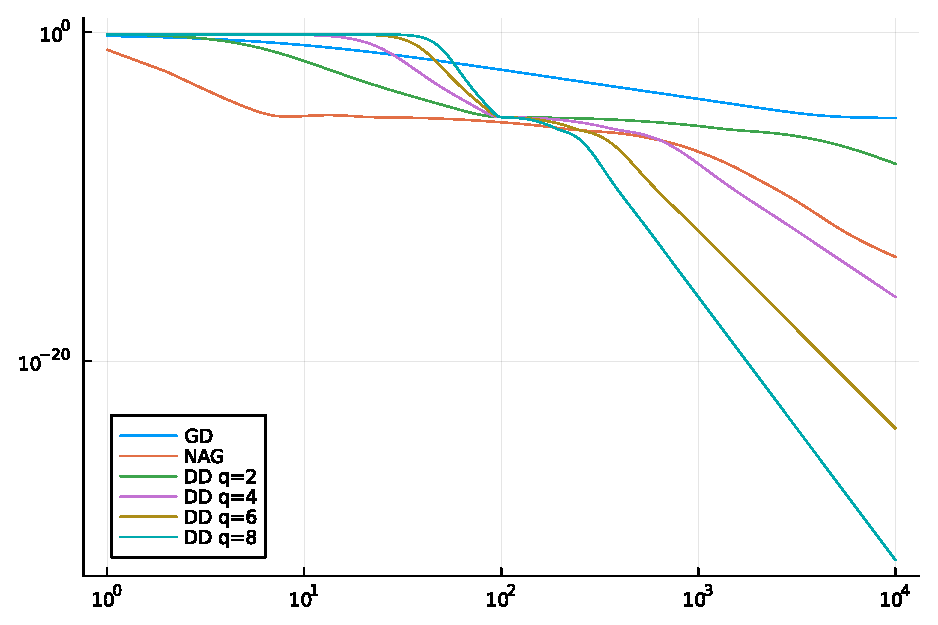
\includegraphics[width=\textwidth]{"assets/l4loss.pdf"}
        \caption{}
        \label{l4}
    \end{subfigure}
    \hfill
    \begin{subfigure}{0.4\textwidth}
        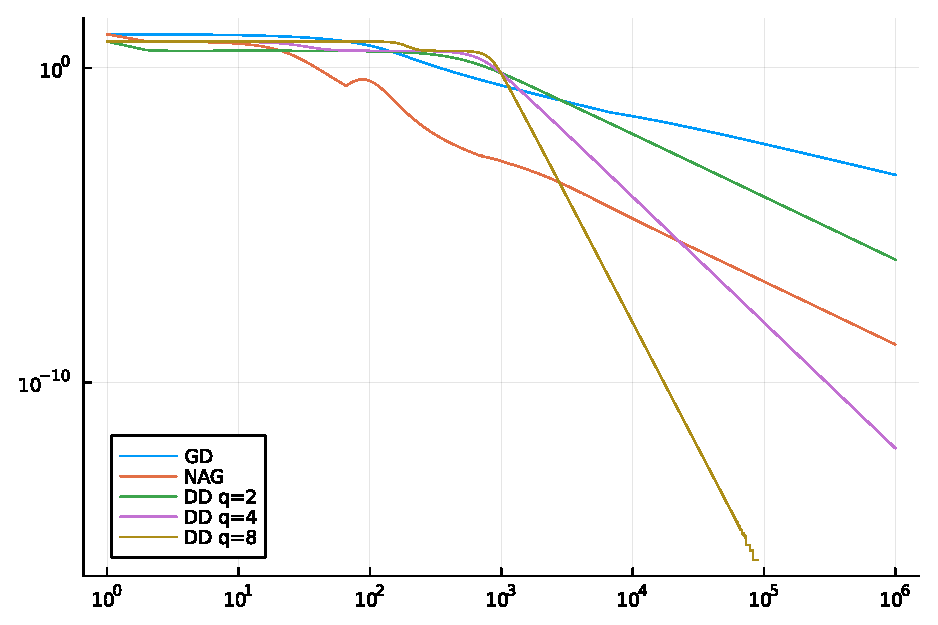
\includegraphics[width=\textwidth]{"assets/logistic.pdf"}
        \caption{}
        \label{fig:logistic}
    \end{subfigure}
    \caption{(a) Convergence}
    \label{Numerical}
\end{figure}